% !TEX root = ../Thesis.tex
\chapter{Design and Implementation of the Artefact} \label{cha:discussion}

\section{Overview of the Artefact}


% The artefact developed in this thesis is a web-based prototype for the Volvo CE Total Market Calculation (TMC) workflow. It is designed to support the workflow from CSV-based upload of source data and matrix files to the execution and inspection of preparation-, adjustment-, and split-related results. In this way, the artefact provides a more transparent and inspectable representation of selected parts of the current SAP-based TMC process.

% The prototype combines three main capabilities. First, it supports structured upload and management of workflow-related input data, including source data and matrix files required for the TMC process. Second, it re-expresses selected parts of the original SAP-based workflow logic through backend processing implemented with Python-based services and SQL-backed data handling. Third, it provides a web-based user interface for reviewing workflow layers, filtering and comparing table data, inspecting updated summary values, and exporting results in CSV format.

% The artefact is implemented as a modular frontend-backend system. The frontend supports navigation, interaction, and result inspection, while the backend handles data ingestion, storage, and workflow-related processing. Through this structure, the prototype does not merely display outputs, but supports a complete workflow-oriented process in which users can upload data, trigger processing, inspect intermediate results, and review derived outputs in a more user-oriented environment than the corresponding SAP-based representation.

% In the context of this thesis, the artefact serves as the main design contribution. It demonstrates how a web-based prototype can make an enterprise calculation workflow more transparent, inspectable, and easier to use, while remaining extensible for future internal use within Volvo CE.


% The artefact developed in this thesis is a web-based data processing and visualization prototype for the Volvo CE Total Market Calculation (TMC) workflow. It is designed to provide a more transparent, inspectable, and user-friendly representation of the workflow than the corresponding SAP-based process. The implemented scope covers workflow stages from source data upload to preparation, adjustment, and machine line split.

% The prototype supports several core functions. It allows users to upload CSV-based source data and matrix files, process selected workflow logic in the backend, and inspect intermediate and derived outputs through a web interface. In addition, the artefact supports interactive table review, filtering, summary calculation, and CSV export, making it easier for users to validate results and understand how workflow outputs are produced.

% \
% To address the identified gap in transparency, inspectability, and usability in the SAP-based TMC workflow, this thesis develops a web-based data processing and visualization artefact for Volvo CE. The artefact supports key workflow stages from source data upload to preparation, adjustment, and machine line split, while providing a more transparent and user-oriented representation compared to the existing SAP-based environment.

% As illustrated in Figure 5.1, the artefact is implemented as a web-based prototype that integrates CSV-based data upload, backend workflow processing, and interactive frontend inspection. The architecture enables ingestion of source data and matrix files, re-expression of selected SAP-based workflow logic using Python and SQL, and presentation of intermediate and derived outputs through a web interface.

% \begin{figure}[H]
%     \centering
%     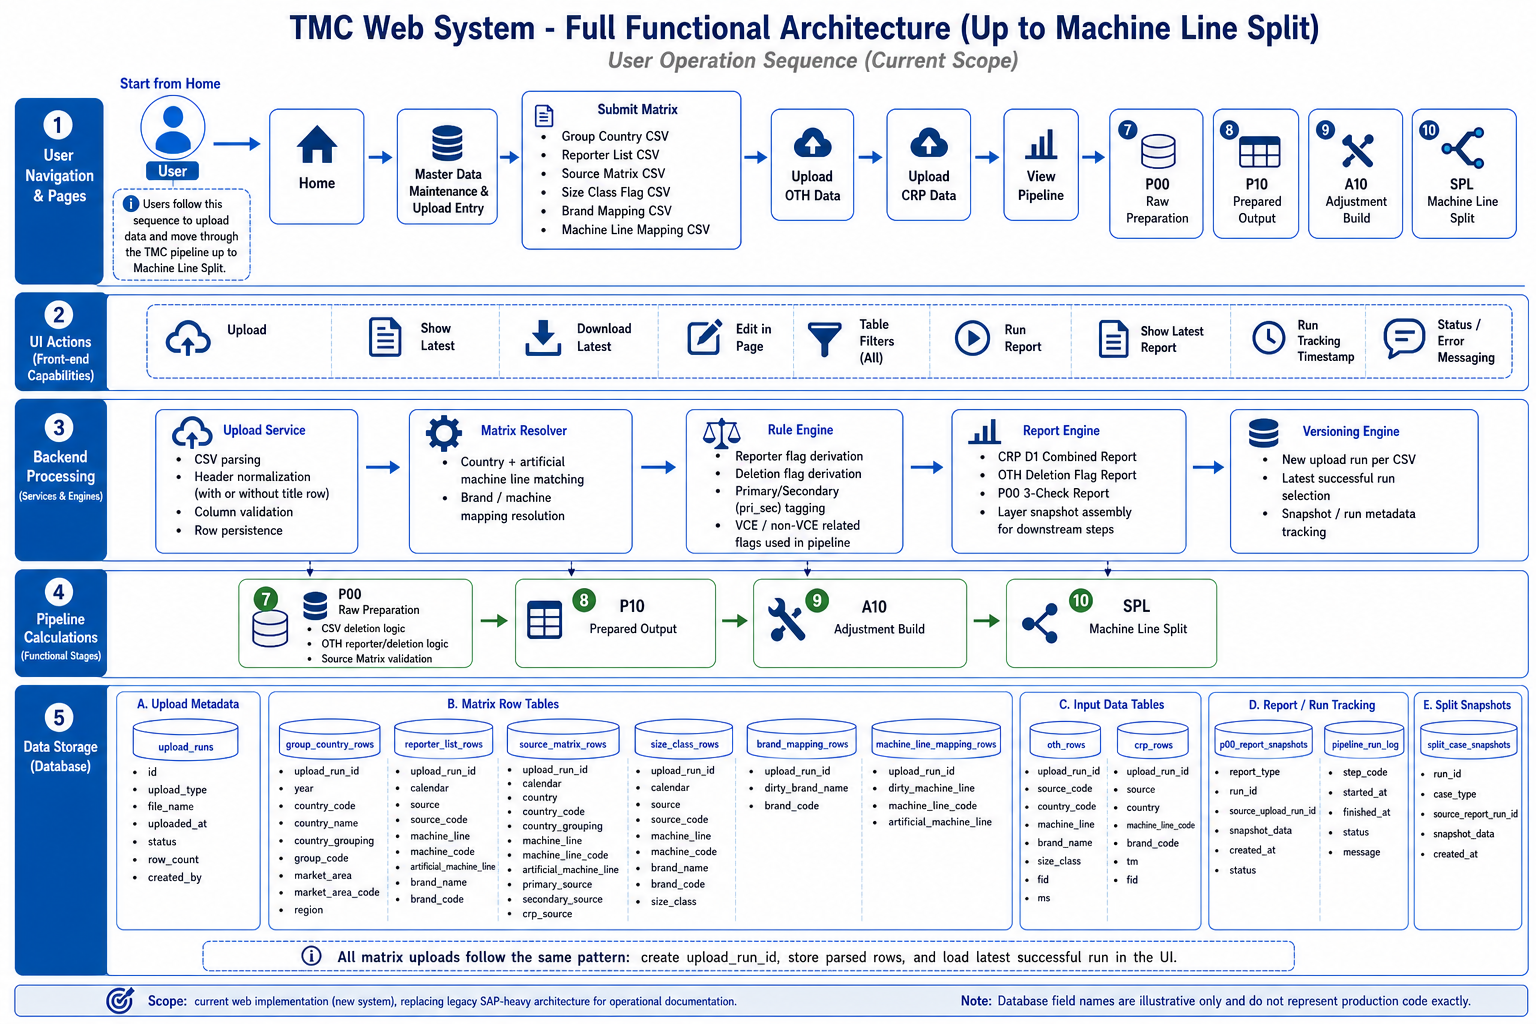
\includegraphics[width=1.0\linewidth]{5.1.png}
%     \caption{ High-level architecture of the web-based TMC artefact}
%     \label{fig:5.1}
% \end{figure}


% The artefact consists of several core elements: (1) support for source data and matrix inputs required in the TMC workflow, (2) backend services that execute workflow logic and organize intermediate and derived outputs, (3) workflow-oriented frontend views for inspecting preparation, adjustment, and split results, and (4) interactive functions such as filtering, summary calculation, and CSV export. Together, these elements form a coherent prototype environment for representing and reviewing selected parts of the TMC workflow in a more transparent and inspectable way.

% In the context of this thesis, the artefact serves as the central design contribution. It demonstrates how parts of a complex enterprise calculation workflow can be transformed into a web-based prototype that improves workflow visibility and user interaction while remaining extensible for future internal use within Volvo CE.



To address the identified gap in transparency, inspectability, and usability in the SAP-based TMC workflow, this thesis develops a web-based artefact for Volvo CE that re-expresses selected parts of the workflow in a browser-accessible environment. The implemented system covers authentication, CSV-based data upload, backend processing, workflow inspection, and review of intermediate and derived outputs for the preparation, adjustment, and machine-line split stages.

The artefact combines a frontend application, backend services, workflow-oriented inspection views, and interactive review functions. Rather than acting only as a reporting interface, it supports a workflow-oriented process in which users can upload data, trigger processing, inspect intermediate results, and review derived outputs within one environment. Together, these elements form a coherent web application for representing and reviewing selected parts of the workflow in a more transparent and inspectable way.


















% \section{Structure and Components of the Artefact}

% \subsection{System Architecture}

% The system architecture of the artefact is shown in Figure 5.1. It illustrates how the prototype is organized into a user interface layer, a backend application layer, and a database layer, together with the flow of uploaded input data, workflow processing, and generated outputs.


% \begin{figure}[H]
%     \centering
%     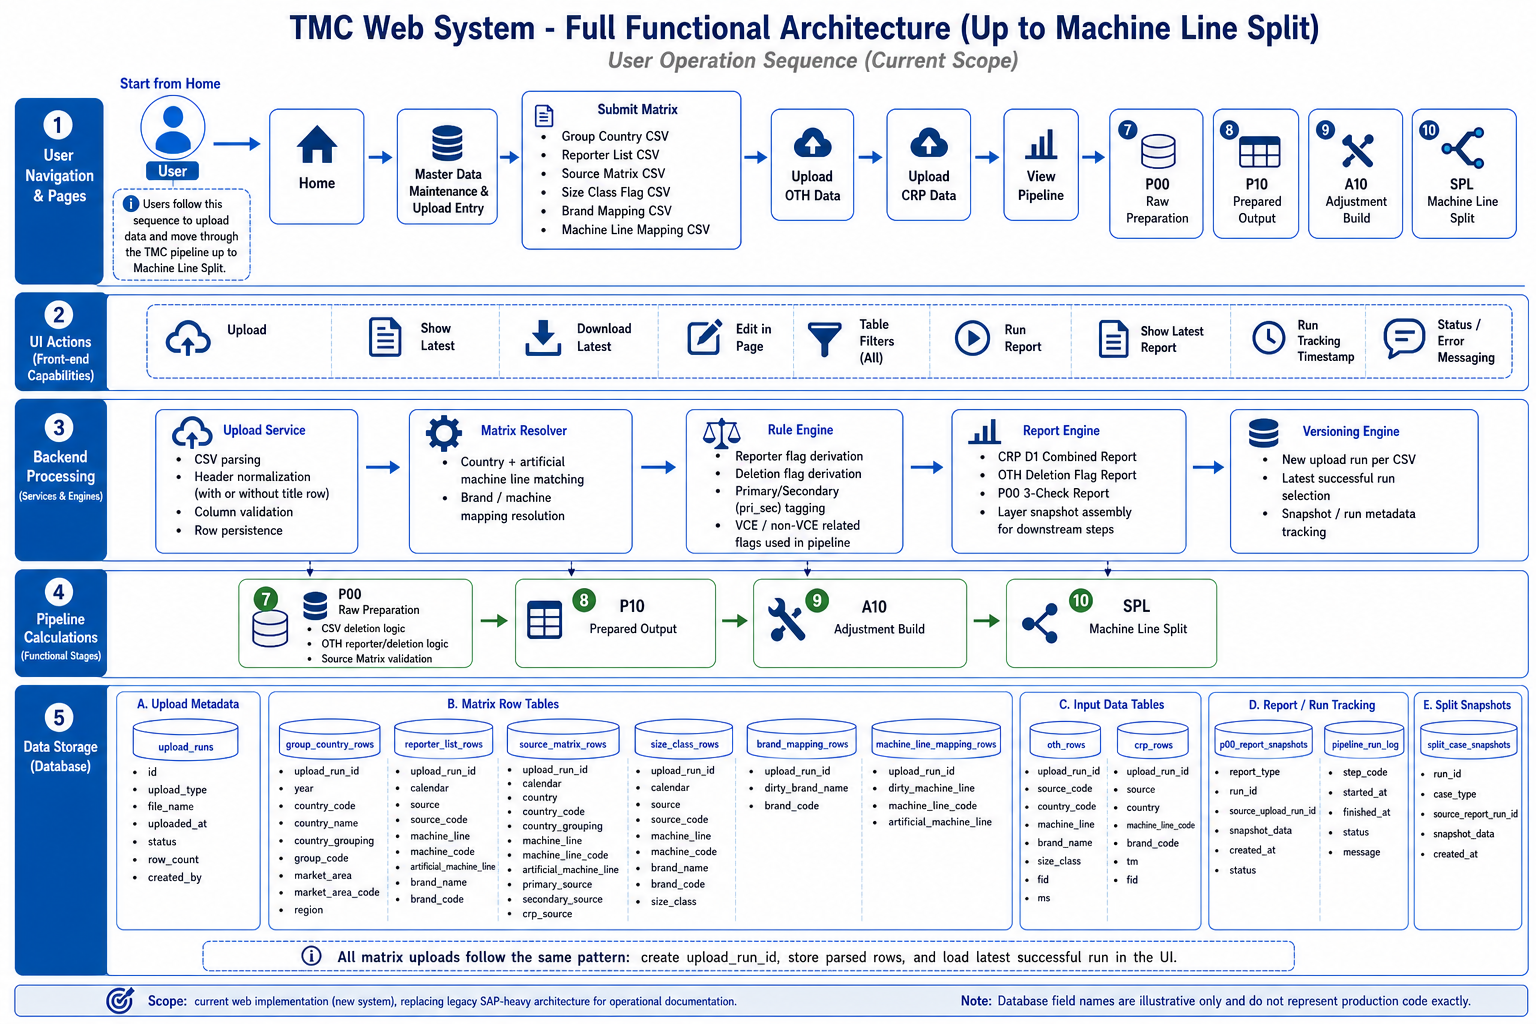
\includegraphics[width=1.0\linewidth]{5.1.png}
%     \caption{ High-level architecture of the web-based TMC artefact}
%     \label{fig:5.1}
% \end{figure}




% On the frontend side, the artefact provides the user interface for navigation, data upload, and inspection of workflow results. This includes views for authentication, homepage-based workflow access, upload of workflow-related CSV files, and layer-based inspection of preparation-, adjustment-, and split-related outputs. The frontend is therefore responsible not only for displaying results, but also for supporting interaction with the workflow in a more transparent and user-oriented way.

% On the backend side, the artefact is implemented through Python-based services that handle file upload, data ingestion, workflow processing, and access to derived outputs. Uploaded files are stored and organized in a structured way, and selected parts of the original SAP-based workflow logic are re-expressed through backend processing supported by SQL-backed storage and querying. This makes it possible to handle workflow-related transformations in a prototype environment that is more inspectable than the original SAP-based representation.

% Between the frontend and backend, the artefact uses API-based communication to transfer uploaded files, request workflow data, and retrieve processed outputs for presentation in the interface. The architecture also includes structured storage for workflow records, mappings, and intermediate outputs, allowing the different workflow stages to be represented in a coherent and modular way.


\section{Overall Design}

\subsection{System Architecture}

The system architecture of the artefact is shown in Figure 5.1. It is organized as a split frontend-backend web application with a persistent data layer, where the frontend provides the user interface, the backend handles authentication and workflow processing, and the database stores uploaded data, session information, and generated outputs. This structure supports browser-based interaction while keeping the implementation modular and easier to maintain.

\begin{figure}[H]
    \centering
    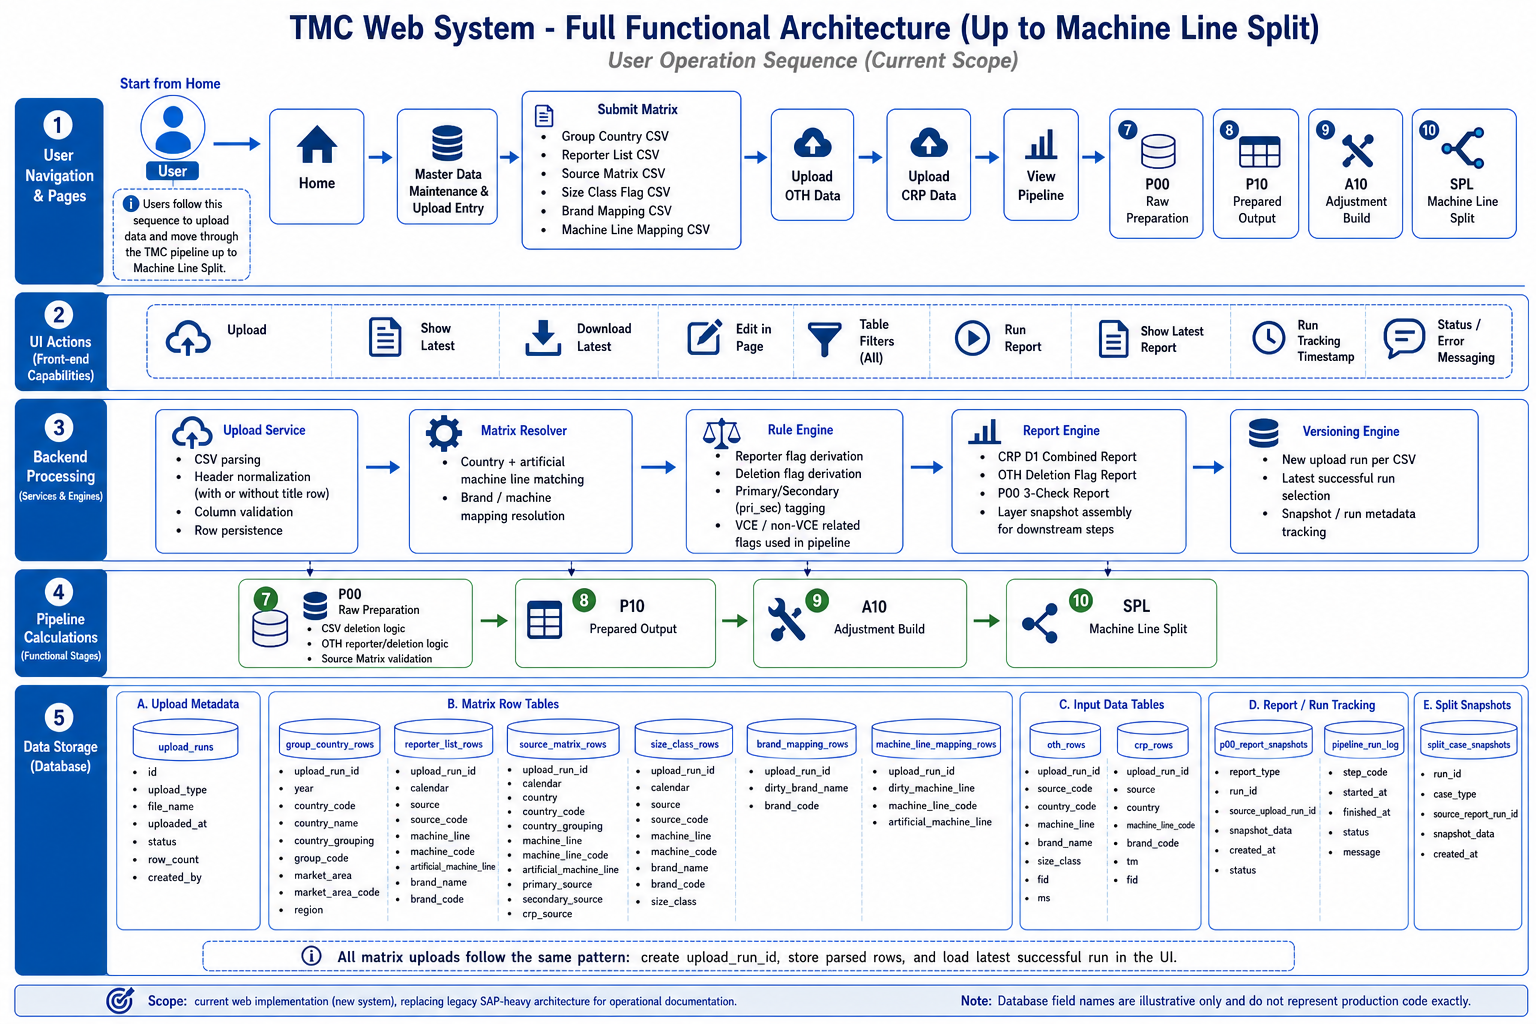
\includegraphics[width=1.0\linewidth]{5.1.png}
    \caption{ High-level architecture of the web-based TMC artefact}
    \label{fig:5.1}
\end{figure}


The frontend is implemented as a single-page application using React and Vite. It uses client-side routing to move between the home page, matrix submission page, upload pages, Pipeline Viewer, and Layer Detail pages. This supports a more interactive review experience.

The backend is implemented with FastAPI and exposes the API endpoints used by the frontend. It also contains the processing logic for the implemented workflow, including file validation, structured storage, and retrieval of intermediate and final outputs.

The data layer is configured through environment variables and supports both SQLite and PostgreSQL. Authentication data is stored separately from the business workflow data, which keeps session management isolated from the calculation data. Communication between the frontend and backend is API-based, so uploaded files, workflow requests, and processed outputs can be exchanged and displayed in structured views such as tables, summaries, and pipeline status cards.




























\subsection{Workflow and Data Flow}

% The execution flow of the artefact follows the staged structure of the implemented TMC workflow. It begins with upload of source data and matrix files and continues through backend cleaning, preparation, adjustment, and split-related processing until the results are exposed in the frontend for inspection.

% The workflow proceeds through the following steps:

% \begin{enumerate}
%     \item \textbf{Upload of source and matrix data.}  
%     Users upload the CSV files required for the workflow through the web interface. In the current prototype, these include source matrix, reporter list, size class, brand mapping, group country, machine line mapping, OTH data, Volvo sales data, and TMA data.

%     \item \textbf{Registration of upload runs.}  
%     Each upload is registered in the \texttt{upload\_runs} table together with metadata such as file name, upload time, status, and row count. This makes it possible to identify the latest successful upload for each data type.

%     \item \textbf{Validation and cleaning in the backend.}  
%     After upload, the files are processed in Python-based backend services. At this stage, the system:
%     \begin{itemize}
%         \item validates the file structure for the selected upload type,
%         \item removes header rows or repeated header-like rows where needed,
%         \item normalizes column names and field values,
%         \item restructures legacy layouts such as the older OTH format,
%         \item standardizes important fields such as size class and size-class mapping.
%     \end{itemize}

%     \item \textbf{Storage in SQL-backed tables.}  
%     The cleaned data is stored in dedicated SQLite tables.
%     \item \textbf{Generation of cleaned intermediate reports.}  
%     Before the main workflow reports are built, the system generates cleaned intermediate outputs:
%     \begin{itemize}
%         \item \texttt{control\_report\_clean\_rows}, which enriches OTH data with mapped country, region, machine line, and brand information,
%         \item \texttt{crp\_tma\_report\_rows}, which aggregates TMA data into a normalized report structure.
%     \end{itemize}

%     \item \textbf{Preparation-stage processing.}  
%     The backend then combines TMA and Volvo sales data into a shared relational structure. At this stage:
%     \begin{itemize}
%         \item TMA data is aggregated into a \texttt{tma\_agg} structure,
%         \item Volvo sales data is aggregated into a \texttt{volvo\_agg} structure,
%         \item country information is resolved from the latest group-country upload,
%         \item artificial machine line is matched from the machine-line mapping upload,
%         \item source matrix logic is used to evaluate country plus artificial-machine-line combinations,
%         \item reporter-list logic is used to assign reporter flags,
%         \item deletion logic is applied to relevant SAL rows.
%     \end{itemize}
%     The main output of this step is the CRP D1 combined preparation report.

%     \item \textbf{P00 and three-check representation.}  
%     The preparation result is then combined with the OTH deletion-flag report to produce the P00 three-check report. This creates one reviewable table containing TMA, SAL, and OTH rows together with matched workflow measures such as TM, VCE FID, and TM Non VCE.

%     \item \textbf{P10 prepared-layer aggregation.}  
%     The preparation output is regrouped into the P10 report. At this stage:
%     \begin{itemize}
%         \item Total Market is calculated from TMA rows,
%         \item VCE is calculated from valid SAL rows with reporter flag \texttt{Y},
%         \item Non-VCE is calculated as \texttt{max(TMA - VCE, 0)}.
%     \end{itemize}

%     \item \textbf{A10 adjustment-stage output.}  
%     The A10 report summarizes SAL and TMA rows into one reviewable result structure for each matched workflow group. It includes detail rows and derived result rows, making the adjustment stage inspectable in the prototype.

%     \item \textbf{Split-related processing.}  
%     The current split-related implementation focuses on excavator split cases. OTH rows are filtered by artificial machine line and size-class conditions, Volvo rows are deducted, and the remaining FID is redistributed using the prepared P10 non-VCE structure as reference. The outputs include both summary rows and detailed split rows.

%     \item \textbf{Frontend inspection and result access.}  
%     The generated outputs are exposed through backend APIs and shown in the frontend as layer-based views, filterable tables, and downloadable results.
% \end{enumerate}

% The final outputs of the artefact therefore include not only uploaded and cleaned datasets, but also staged workflow reports such as the


% The execution flow of the artefact begins with CSV-based upload of the datasets required for the TMC workflow and continues through backend cleaning, preparation, adjustment, and split-related processing until the resulting outputs are made available in the frontend.

% The main execution logic can be summarized as follows:

% \begin{itemize}
%     \item \textbf{CSV upload.}  
%     The workflow starts when users upload the required CSV files through the web interface. In the current prototype, these inputs include source matrix, reporter list, size class input, brand mapping, group country, machine line mapping, OTH data, Volvo sales data, and TMA data.

%     \item \textbf{Validation and cleaning of uploaded data.}  
%     After upload, the backend validates the file structure and performs dataset-specific cleaning. This includes removal of header rows or repeated header-like rows, handling of layout variations, normalization of textual values, and standardization of important fields such as size class. The cleaned CSV content is then transformed into a consistent internal structure.

%     \item \textbf{Generation of cleaned source-level data.}  
%     The cleaned inputs are reorganized into structured source-level outputs. OTH data is combined with country, machine-line, and brand-related mapping data, while TMA data and Volvo sales data are prepared in forms that can be aligned in later workflow stages.

%     \item \textbf{Preparation-stage processing.}  
%     In the preparation stage, the cleaned source datasets are brought into a shared workflow structure. At this stage, country mapping, artificial machine-line mapping, source-related logic, and reporter-related logic are applied in order to generate the first workflow-oriented outputs. The result of preparation is therefore an inspectable structure in which TMA and Volvo sales records can be reviewed together with the relevant workflow flags and aligned dimensions.

%     \item \textbf{Preparation outputs.}  
%     The preparation stage produces:
%     \begin{itemize}
%         \item a preparation-layer output for TMA and Volvo sales related records,
%         \item a cleaned OTH-oriented output with mapped workflow fields,
%         \item a combined review output that brings together TMA, SAL, and OTH-related rows in one inspectable structure.
%     \end{itemize}

%     \item \textbf{Prepared market-view output.}  
%     After preparation, the prototype derives a more compact market-oriented output in which the main workflow measures are summarized. At this stage, the system presents total market, Volvo CE-related values, and non-Volvo CE-related values in a form suitable for review.

%     \item \textbf{Adjustment-stage processing.}  
%     The adjustment stage reorganizes the prepared results into a reviewable adjustment-oriented structure. In the current implementation, this stage makes it possible to inspect both source-detail rows and the derived result rows for the same workflow group.

%     \item \textbf{Split-related processing.}  
%     The split stage redistributes grouped OTH values into more detailed output structures. In the implemented split cases, the starting point is an OTH row whose machine-line category is broader than the intended final output. The prototype therefore uses the prepared market-view result as a reference basis for split.

%     \item \textbf{How split ratios are determined.}  
%     The split ratio is derived from the non-Volvo CE distribution in the prepared output. For a broader grouped value, the system identifies the relevant smaller target buckets and calculates each ratio as the reference value of that bucket divided by the sum of the relevant reference values. The original OTH value is then multiplied by these ratios in order to obtain the split results. When detailed reference data is not available at country level, the current implementation applies a fallback logic through broader aggregation levels.

%     \item \textbf{Final outputs.}  
%     The final outputs are not limited to one single result table. Instead, the artefact produces a sequence of staged outputs, including cleaned source-level outputs, preparation-layer outputs, combined review outputs, prepared market-view results, adjustment-stage results, and split-related results. These are displayed in the frontend as workflow-layer views, filterable tables, summary values, and downloadable results.
% \end{itemize}


The execution flow of the artefact begins with browser-based upload of the datasets required for the TMC workflow and continues through backend validation, cleaning, persistence, processing, and frontend inspection. Each upload is registered together with metadata such as file name, upload time, status, and row count. This makes it possible to identify the latest valid input for each data type and to trace how the workflow was executed.


\begin{figure}[H]
    \centering
    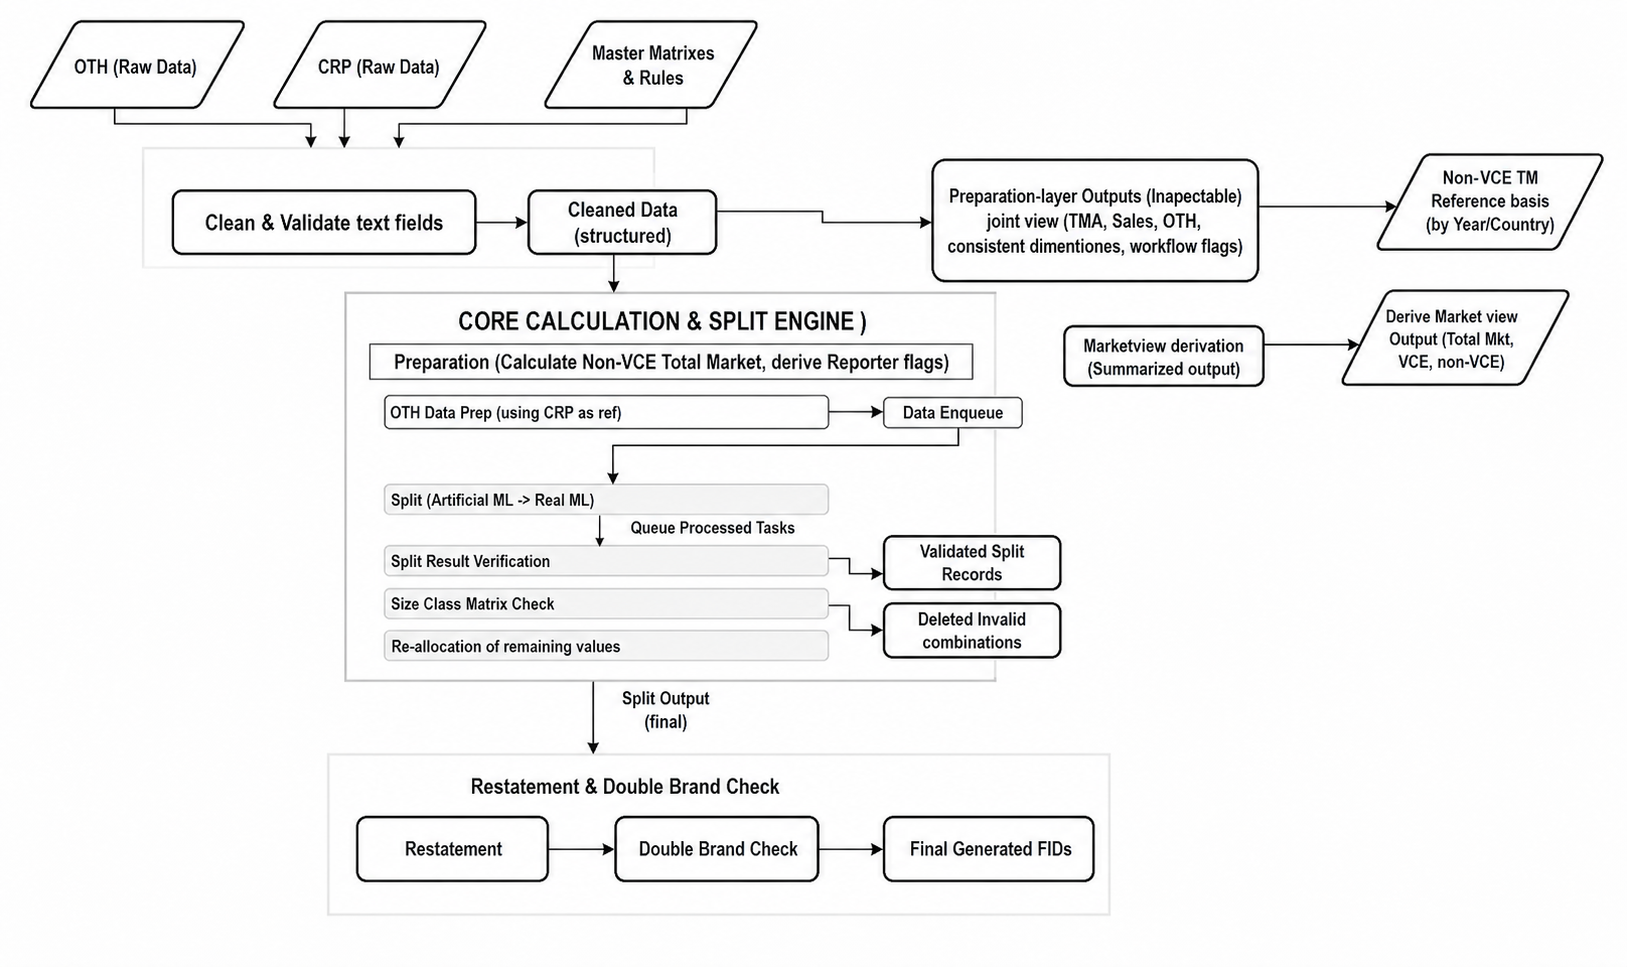
\includegraphics[width=1.2\linewidth]{5.2.1.png}
    \caption{Data Flow and Processing Stages of the TMC Artefact}
    \label{fig:5.2}
\end{figure}







\begin{itemize}
    \item \textbf{CSV upload and validation.}  
    The workflow starts with users uploading the required source and matrix files through the web interface. The backend validates file structure and performs dataset-specific cleaning, such as removing header rows, normalising textual values, and standardising key fields.

    \item \textbf{Source-level data preparation.}  
    The cleaned inputs are transformed into structured source-level data. OTH data is combined with mapping tables, while TMA and Volvo sales data are prepared for alignment in subsequent stages.

    \item \textbf{Preparation stage.}  
    In this stage, datasets are aligned within a shared workflow structure. Country mapping, artificial machine-line mapping, source logic, and reporter determination are applied to produce inspectable preparation-layer outputs that bring TMA, Volvo sales, and OTH data into consistent dimensions.

    \item \textbf{Market-view derivation.}  
    A summarized market-oriented output is derived from the preparation results, presenting total market, Volvo CE values, and non-Volvo CE values in a compact and reviewable form.

    \item \textbf{Adjustment stage.}  
    The adjustment stage reorganizes the prepared data into a structure that allows inspection of both source-level records and derived results within the same workflow context.

    \item \textbf{Split processing.}  
    The split stage redistributes grouped OTH values into more detailed categories. The prepared market-view output is used as a reference basis, and split ratios are derived from the non-Volvo CE distribution. When detailed reference data is unavailable at country level, fallback logic based on higher-level aggregation is applied.

    \item \textbf{Final outputs and presentation.}  
    The artefact produces multiple staged outputs, including cleaned data, preparation-layer outputs, adjustment results, and split results. These are presented in the frontend as workflow views, filterable tables, summary metrics, and downloadable files.
\end{itemize}




% \section{Functions and Behaviour of the Core Component}


\section{Detail Design}

% \subsection{CSV Upload and Input Handling}



% A central function of the artefact is to support structured upload of workflow-related CSV files through the web interface. The upload and input-handling component provides the data foundation for the subsequent workflow stages.

% The uploaded inputs in the current prototype can be grouped into the following categories:

% \begin{itemize}
%     \item market-related source data CSV,
%     \item sales-related source data CSV,
%     \item reference market data CSV,
%     \item source-definition matrices CSV,
%     \item reporter and mapping inputs CSV,
%     \item country and grouping definitions CSV,
%     \item machine-line and size-class-related mapping data CSV.
% \end{itemize}

% These inputs have different roles in the workflow. Some provide the market and sales values that are processed in later stages, while others define how the source records should be aligned, grouped, interpreted, and redistributed.

% After upload, each file is registered together with metadata such as upload type, file name, upload time, status, and row count. This allows the prototype to identify the latest successful version of each required input and use it as the basis for later workflow execution.

% The uploaded data is finally reflected in the artefact through:

% \begin{itemize}
%     \item upload views showing whether the required input categories are available,
%     \item result views showing upload status and basic upload information,
%     \item workflow-layer views in which the uploaded inputs are transformed into preparation-, adjustment-, and split-related outputs.
% \end{itemize}



\subsection{CSV Upload and Input Handling}

A central function of the artefact is to support structured upload of workflow-related CSV files through the web interface. This component provides the data foundation for the later workflow stages and is accessed through dedicated frontend entry points such as the matrix submission page, upload pages, the Pipeline Viewer, and Layer Detail views.

The uploaded inputs in the current prototype can be grouped into market data, sales data, reference market data, source-definition matrices, and mapping-related inputs such as reporter, country, machine-line, and size-class definitions.

After upload, each file is registered with metadata such as upload type, file name, upload time, status, and row count. This allows the prototype to identify the latest successful version of each required input and use it as the basis for later workflow execution and inspection.

The uploaded data is then reflected in upload views, result views, and workflow-stage views.

























 % \subsection{Data Cleaning and Workflow Preparation}



% The preparation stage is the first workflow-oriented processing stage in the artefact. Its purpose is to transform the uploaded source data and mapping input into structured results that can be reviewed before later adjustment and split-related processing.

% The main functions of this stage are:

% \begin{itemize}
%     \item aligning uploaded source records with the relevant workflow definitions, including country-related grouping logic, machine-line-related mapping, source definitions, and reporter-related input,
%     \item assigning workflow control fields such as deletion flag, reporter flag, and source-related preparation indicators,
%     \item reorganizing source records from different origins into a shared workflow structure,
%     \item generating preparation-level outputs that can be inspected before later workflow stages are applied.
% \end{itemize}

% For OTH-related records, the preparation stage includes the following processing:

% \begin{itemize}
%     \item the uploaded rows are first aligned with country, machine-line, and brand-related mappings,
%     \item rows that belong to the same mapped workflow combination are then aggregated and their values are summed into preparation-ready results,
%     \item the resulting structured rows are used as the OTH-oriented preparation output for later review and downstream workflow processing.
% \end{itemize}

% For TMA- and sales-related records, the preparation stage produces a comparable workflow representation in which different source categories can be reviewed together. This makes it possible to inspect the data in a shared structure instead of as isolated uploaded files.

% The outputs of this stage are reflected in the artefact through preparation-layer views and combined review-oriented results. These outputs provide the first inspectable representation of how uploaded input data is transformed inside the prototype and serve as the basis for the later market-view, adjustment, and split-related stages.



\subsection{Preparation Stage}

% The preparation stage is the first workflow-oriented processing stage in the artefact. Its purpose is to transform uploaded source data and mapping input into structured results that can be reviewed before later adjustment and split and resplit processing.

% The preparation stage in the current prototype consists of the following main steps. Together, these steps make early workflow transformations visible before later market-view, adjustment, and split-related processing is applied:

% \begin{itemize}
%     \item \textbf{OTH-oriented preparation.}  
%     Uploaded OTH rows are first aligned with country-related grouping input, machine-line mapping, brand mapping, source matrix, and reporter-related input. After this alignment, the artefact assigns preparation control fields such as deletion flag, Pri/Sec, and reporter flag. Rows that belong to the same mapped workflow combination are then aggregated and their values are summed into a structured OTH-oriented preparation output.

%     \item \textbf{CRP/TMA/SAL-oriented preparation.}  
%     TMA and sales-related records are reorganized into a shared workflow structure. At this stage, the artefact applies country mapping, artificial machine-line mapping, source-matrix-related logic, and reporter-related matching in order to produce preparation-level records. The resulting output makes it possible to review TMA- and sales-related source categories together within one comparable structure.

%     \item \textbf{Assignment of workflow control logic.}  
%     A central function of the preparation stage is to make workflow logic explicit in the artefact. In the current implementation, this includes preparation-related fields such as deletion flag and reporter flag, together with source-related classification logic used for later workflow interpretation.

%     \item \textbf{Combined preparation review output.}  
%     After the OTH-oriented and CRP/TMA/SAL-oriented preparation outputs have been generated, the artefact produces a combined review-oriented result in which TMA, SAL, and OTH-related rows can be inspected within a shared workflow view. This gives the user an early overview of how the uploaded input data has been transformed before later stages are applied.
% \end{itemize}

% The outputs of this stage are reflected in the artefact through preparation-layer views and review-oriented tables. These outputs provide the basis for the later market-view, adjustment, and split-related stages, while also allowing users to inspect the preparation logic in a more explicit and transparent way than in the original SAP-based environment.




The preparation stage is the first workflow-oriented processing stage in the artefact. Its purpose is to transform uploaded source data and mapping input into structured results that can be reviewed before later adjustment and split and resplit processing.

The preparation stage in the current prototype consists of the following main steps. Together, these steps make early workflow transformations visible before later market-view, adjustment, and split-related processing is applied:

\begin{itemize}
    \item \textbf{OTH-oriented preparation.}  
    Uploaded OTH rows are aligned with country-related grouping input, machine-line mapping, brand mapping, source matrix, and reporter-related input. During this step, backend logic assigns preparation control fields such as deletion flag, Pri/Sec, and reporter flag. Rows that belong to the same mapped workflow combination are then aggregated into a structured OTH-oriented preparation output.

    \item \textbf{CRP/TMA/SAL-oriented preparation.}  
    TMA and sales-related records are reorganised into a shared workflow structure through SQL-based grouping, joins, and aggregation. Country mapping, artificial machine-line mapping, source-matrix logic, and reporter-related matching are applied to produce preparation-level records that can be reviewed together.

    \item \textbf{Combined preparation review output.}  
    After the OTH-oriented and CRP/TMA/SAL-oriented preparation outputs have been generated, the artefact exposes them through backend APIs and renders them in workflow views. This produces a combined review-oriented result in which TMA, SAL, and OTH-related rows can be inspected before later stages are applied.
\end{itemize}






% \subsection{Adjustment and Split Stage}



% After the preparation stage, the artefact represents the subsequent workflow through adjustment-oriented and split-related outputs. This component is implemented through React-based frontend views, FastAPI endpoints, and SQL-backed backend processing.

% The main functions of this component are:

% \begin{itemize}
%     \item reorganizing prepared TMA- and SAL-related rows into adjustment-oriented result structures,
%     \item generating source-detail rows together with derived result rows for the same workflow group,
%     \item applying split-related logic to selected grouped OTH values,
%     \item exposing both adjustment and split-related outputs through reviewable frontend views.
% \end{itemize}

% In the adjustment stage, the backend groups the prepared workflow data along shared workflow dimensions and generates an output that includes SAL detail rows, TMA detail rows, and one derived result row for each matched workflow group. This makes it possible to inspect how the adjusted result is formed from the prepared records rather than only showing a final aggregated value.

% In the split-related stage, the backend combines prepared OTH-oriented data with the prepared market-view output. Grouped OTH values are filtered, Volvo-related values are deducted, and split ratios are derived from the prepared non-Volvo CE distribution in order to redistribute the remaining value into more detailed result structures.

% The resulting outputs are returned through backend APIs and rendered in the frontend as workflow-layer views and filterable tables. In this way, the artefact makes the later workflow stages both executable in the backend and inspectable in the frontend.



\subsection{Adjustment and Split Stage}

After preparation, the artefact continues with adjustment-oriented and split and resplit processing.

The main functions of this component are:
\begin{itemize}
    \item regrouping prepared TMA and SAL rows into adjustment outputs,
    \item splitting grouped OTH values into more detailed machine-line and size-class buckets,
    \item calculating split ratios from the prepared non-Volvo CE distribution,
    \item supporting resplit and manual correction for selected split cases.
\end{itemize}

The adjustment stage produces an intermediate review result organised around shared workflow keys such as country and machine line. In this output, TMA and SAL rows for the same country and machine line are brought together, making it easier to inspect how the adjusted result is formed.

The split stage is needed because uploaded OTH data is not always available at the granularity required by the workflow. In this stage, aggregated OTH values are redistributed into smaller target buckets using split ratios derived from a non-Volvo CE reference distribution. The prepared market-view output provides the reference basis, with Volvo CE sales excluded before proportional ratios are calculated.

For selected cases, the prototype also supports a resplit step that recalculates the split using source-matrix and size-class mappings before the resulting rows are saved. This step is needed because some brands may be active in a country and machine line, but not in all size classes within that market. In such cases, the prototype uses the source matrix and size-class matrix to determine valid size classes and reallocate values from invalid brand--machine-line--size-class combinations to valid target buckets.

The resulting outputs are returned through backend APIs and rendered in the frontend as workflow-stage views and filterable tables. In this way, the implemented adjustment and split and resplit stages are both executable in the backend and inspectable in the frontend.















% \subsection{Visualization and Interaction}

% The visualization and interaction layer presents workflow results through the React-based frontend. In the current prototype, backend-generated outputs are shown through summary-oriented dashboard views, chart-based representations, and filterable tables.

% This layer supports both overview and detailed inspection. Dashboard elements and charts provide a compact view of selected workflow values, while table-based views allow users to inspect the underlying rows in a way that is closer to spreadsheet-based work. Users can filter the displayed data, review grouped values, and inspect summary calculations directly in the interface. In particular, after filtering, the interface can display the summed values of the filtered result set at the top of the table view, which supports quick validation and comparison.

% The component also supports CSV export of selected results. This allows workflow outputs to be downloaded for further review and analysis outside the artefact. In this way, the visualization layer combines dashboard-style presentation, spreadsheet-like inspection, dynamic summary feedback, and export functionality in one web-based environment.


\subsection{Visualization and Interaction}

The visualization and interaction layer presents uploaded data and workflow results through the React-based frontend. In the current prototype, backend-generated outputs and uploaded inputs are shown through workflow-specific views such as the Pipeline Viewer, Layer Detail pages, upload result pages, and table-based inspection views.

This layer supports both overview and detailed inspection. The Pipeline Viewer provides a compact view of the overall workflow status, while the Layer Detail pages allow users to inspect the underlying rows in a way that is closer to spreadsheet-based work. Users can filter the displayed data, review grouped values, and inspect summary calculations directly in the interface. In addition, uploaded data can be edited directly on the page and saved for later workflow steps, which allows small corrections to be made without returning to the original CSV files.

The component also supports CSV export of selected results. This allows workflow outputs to be downloaded for further review and analysis outside the artefact. In this way, the visualization and interaction layer combines workflow overview, row-level inspection, editable uploaded data, dynamic summary feedback, and export functionality in one web-based environment.








% \section{Development Process}



% % The prototype was developed incrementally as a full-stack web application. Rather than implementing the final workflow output directly, development first focused on the technical infrastructure required for authenticated access, page-based navigation, CSV upload, structured storage, and staged report generation. This provided the basis for the later implementation of workflow-specific logic and frontend inspection.

% % The system was implemented with a React- and TypeScript-based frontend and a Python/FastAPI-based backend. The frontend was built with Vite and React Router, which enabled the prototype to be organized into dedicated pages for authentication, upload, workflow navigation, and layer-based inspection. An authentication context was introduced in React to manage login state and protected routes, while a dedicated API client layer connected frontend pages to backend endpoints in a consistent way.

% % \begin{figure}[h]
% %     \centering
% %     % Insert grouped frontend screenshots, e.g. auth page, upload page, layer detail page, filtered table view
% %     \caption{Selected frontend views developed during the implementation of the prototype}
% %     \label{fig:development_frontend_views}
% % \end{figure}

% % On the backend side, FastAPI was used to implement the application service layer. At startup, the backend initializes both the workflow database and the authentication database. Separate routers were implemented for authentication and workflow-related upload/report functionality. The authentication part handles registration, login, session creation, and protected API access, while the workflow router exposes upload, report, and result retrieval endpoints for the frontend.

% % The next major implementation step was CSV upload and relational storage. Uploaded files are submitted from the React upload pages to the FastAPI upload endpoint together with their dataset type. In the backend, dataset-specific Python handlers process each upload according to its role in the workflow. At this stage, \texttt{pandas} is used to read heterogeneous CSV files, remove header rows or repeated header-like rows, handle layout differences, normalize field names and values, and transform the content into a consistent internal structure. The cleaned rows are then stored in SQLite tables, while upload metadata such as file type, file name, upload time, row count, and processing status is stored separately in an upload tracking table.

% % After the upload layer had been completed, development focused on report generation. The first implemented report endpoints produced cleaned source-level outputs for uploaded OTH and TMA data. These reports were generated from the latest successful uploads and were used to verify that source datasets had been parsed and structured correctly before the workflow stages themselves were implemented.

% % \begin{figure}[h]
% %     \centering
% %     % Insert figure or screenshot showing upload-to-preparation processing
% %     \caption{Implementation of CSV upload, cleaning, and preparation-stage report generation}
% %     \label{fig:development_preparation_reports}
% % \end{figure}

% % The preparation stage was implemented next as the first workflow-oriented report layer. Technically, this stage combines Python-based backend orchestration with SQL-based joins, filtering, and aggregation over the stored relational tables. Uploaded source records are aligned with country grouping, machine-line mapping, source matrix logic, and reporter-related input. Workflow control fields such as deletion flag, reporter flag, and source-related classification indicators are generated explicitly in the backend output. For OTH-related records, mapped rows are aggregated into preparation-ready results, while TMA- and sales-related records are reorganized into a shared workflow structure that can later be inspected together.

% % After preparation had been established, the backend was extended with prepared and adjustment-oriented result generation. SQL-based grouped queries were used to regroup preparation results into more compact and reviewable report structures. A key implementation decision at this stage was that the API should not return only one final value table. Instead, the adjustment-oriented output was designed to include both source-detail rows and derived result rows for the same workflow group, so that the frontend could expose how the resulting values are formed.

% % The next implementation step was split-related processing. In the current prototype, this stage combines prepared OTH-oriented outputs with prepared market-view outputs. Python-based backend logic coordinates the execution flow, while SQL-derived grouped reference values are used to determine redistribution ratios. The resulting output includes summary rows, detailed split rows, and supporting reference information, allowing the split logic to be inspected in the frontend rather than remaining hidden as a backend-only calculation.

% % \begin{figure}[h]
% %     \centering
% %     % Insert screenshot showing adjustment or split-related result view
% %     \caption{Implementation of adjustment- and split-related workflow views}
% %     \label{fig:development_adjustment_split_views}
% % \end{figure}

% % Frontend development progressed together with these backend reports. Once the report endpoints were available, the layer detail page was extended to request report data through the API client layer and render the returned JSON results in workflow-specific views. A reusable filterable table component was implemented so that different layers could share the same table logic. This component supports column-based filtering, row counting, and dynamic recalculation of numeric sums for the filtered result set. In addition, summary cards, chart-based representations, and CSV export functionality were added so that users can move between high-level overview and row-level inspection within the same interface.



% The prototype was developed incrementally as a full-stack web application. Instead of implementing the final workflow output directly, development first established the technical infrastructure required for authentication, page navigation, CSV upload, structured storage, and staged report generation. This provided the foundation for later workflow-specific logic and frontend inspection.

% The system consists of a React- and TypeScript-based frontend and a Python/FastAPI-based backend. The frontend, built with Vite and React Router, is organized into pages for authentication, upload, workflow navigation, and layer-based inspection. An authentication context manages login state and protected routes, while an API client layer enables consistent communication with backend endpoints.

% \begin{figure}[H]
%     \centering
%     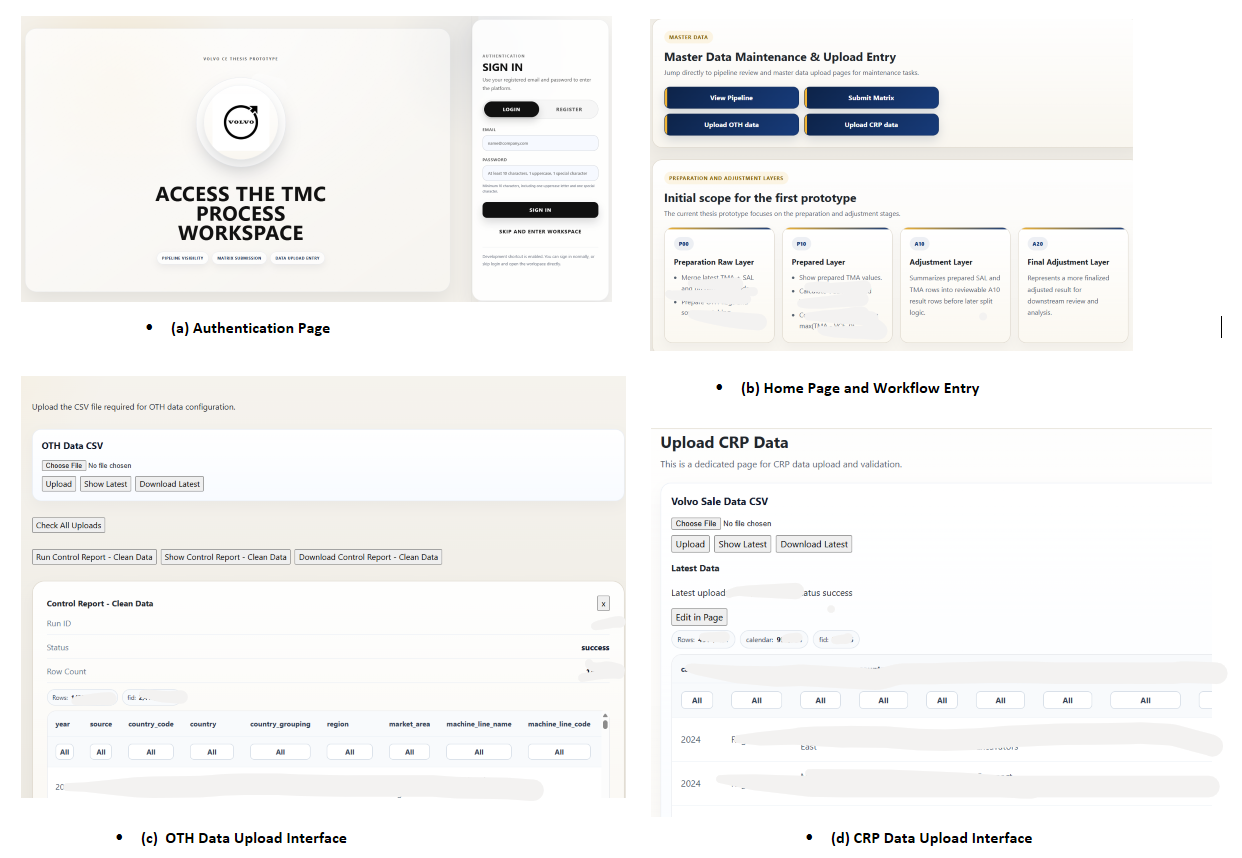
\includegraphics[width=1.0\linewidth]{5.3.png}
%     \caption{Selected frontend views developed during the implementation of the prototype}
%     \label{fig:5.3}
% \end{figure}






% On the backend, FastAPI implements the service layer, with SQLite used for relational storage. At startup, the system initializes workflow and authentication databases, and defines separate routers for authentication and workflow-related functionality. These include endpoints for upload, report generation, and result retrieval.

% The next step focused on CSV upload and data storage. Files are submitted from the frontend together with dataset type information and processed by dataset-specific Python handlers. Using \texttt{pandas}, heterogeneous CSV files are parsed, cleaned, and normalized into a consistent structure. The processed rows are stored in SQLite tables, while upload metadata is tracked separately.

% Once the upload layer was established, development moved to report generation. Initial endpoints produced cleaned source-level outputs for OTH and TMA data, enabling validation of parsing and data alignment.

% \begin{figure}[H]
%     \centering
%     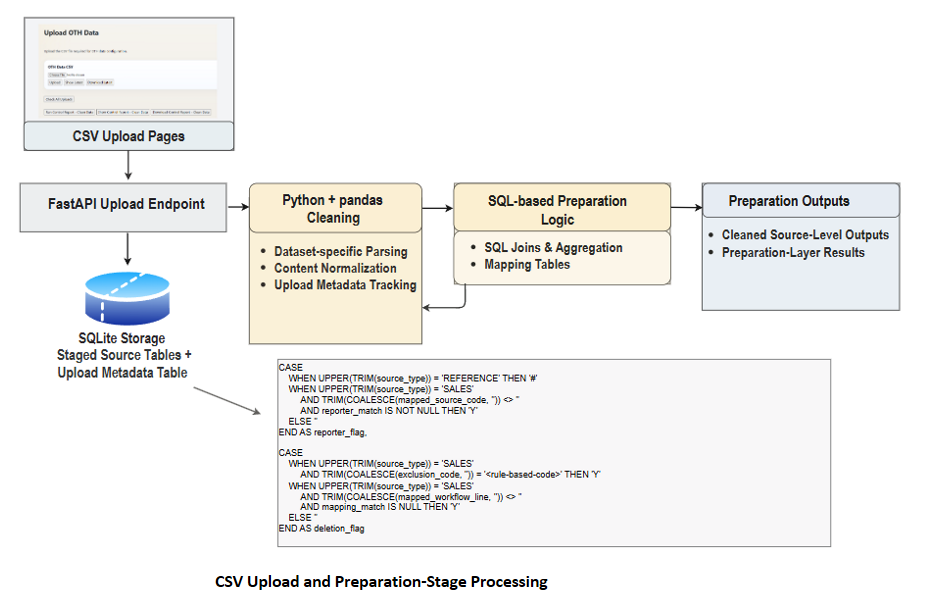
\includegraphics[width=1.0\linewidth]{5.4.png}
%     \caption{Implementation of CSV Upload and Preparation-Stage Processing}
%     \label{fig:5.4}
% \end{figure}



% \begin{figure}[H]
%     \centering
%     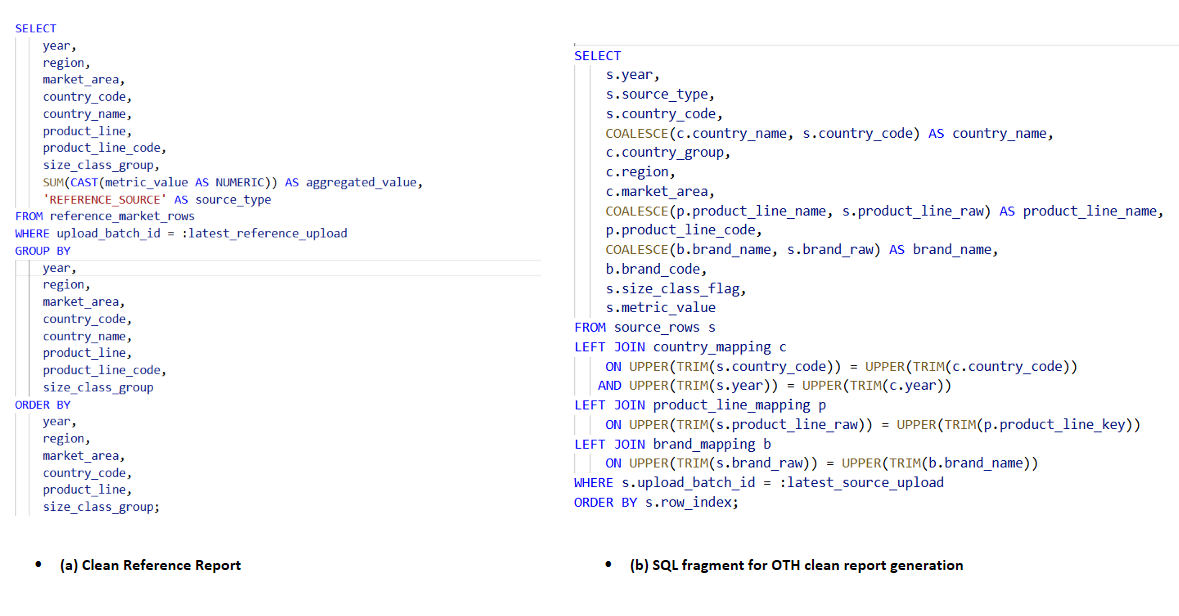
\includegraphics[width=1.0\linewidth]{5.4.1.png}
%     \caption{ Simplified SQL Fragments for CRP/TMA and OTH Clean Report Generation}
%     \label{fig:5.4.1}
% \end{figure}





% The preparation stage was then implemented using SQL-based joins, filtering, and aggregation over stored tables. Source records are aligned with mapping data and enriched with workflow control fields such as deletion and reporter flags. The resulting outputs provide a consistent structure for joint inspection of TMA, sales, and OTH data.

% Subsequently, adjustment and prepared result layers were introduced through grouped SQL queries. A key design decision was to return both source-detail rows and derived results within the same output, allowing the frontend to expose how final values are constructed.

% The split stage was implemented by combining prepared OTH data with market-view outputs. Backend logic coordinates the execution, while SQL-derived reference values are used to calculate redistribution ratios. The resulting outputs include summary rows, detailed split results, and supporting reference values, enabling the split logic to be inspected rather than hidden.



% \begin{figure}[H]
%     \centering
%     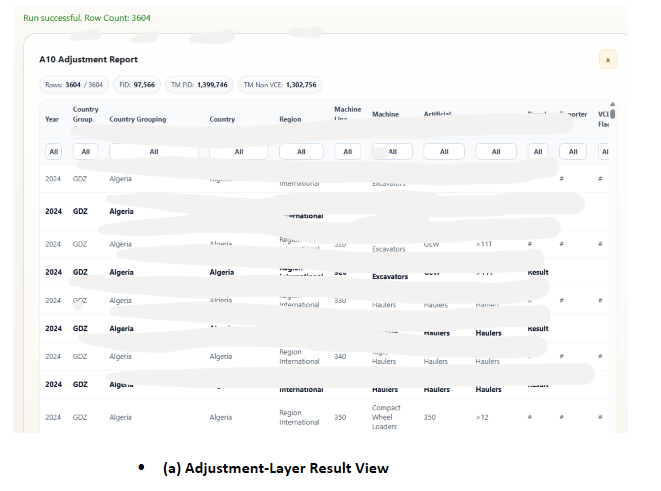
\includegraphics[width=0.9\linewidth]{5.6.1.png}
%     % \caption{Implementation of adjustment- and split-related workflow views}
%     \label{fig:5.6.1}
% \end{figure}





% \begin{figure}[H]
%     \centering
%     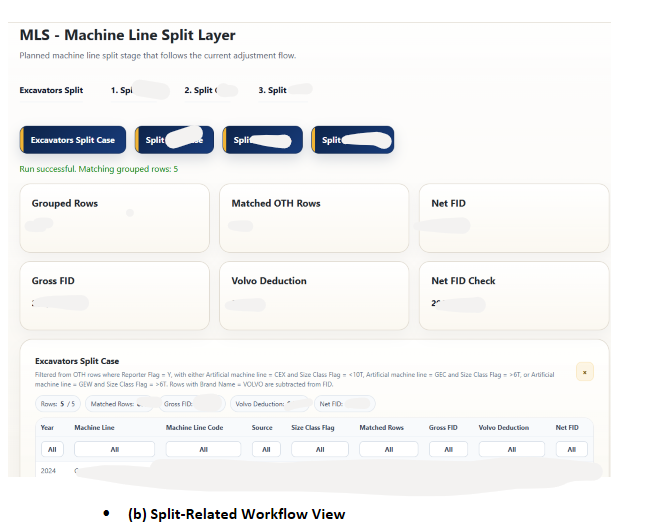
\includegraphics[width=0.9\linewidth]{5.6.2.png}
%     \caption{Implementation of adjustment- and split-related workflow views}
%     \label{fig:5.6.2}
% \end{figure}


% \begin{figure}
%     \centering
%     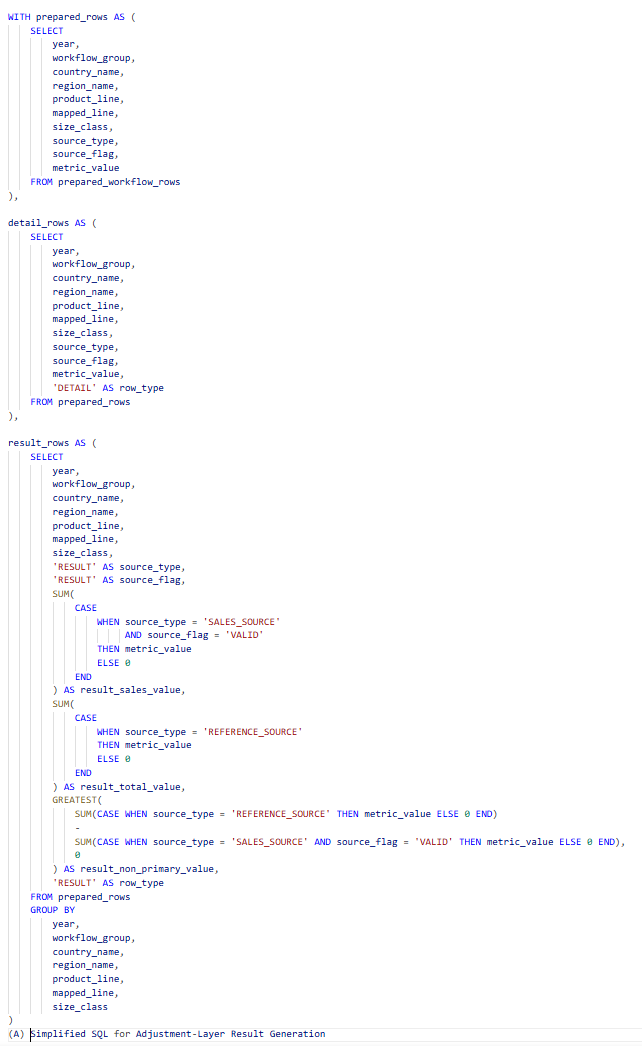
\includegraphics[width=1.1\linewidth]{5.6.3.png}
%     % \caption{Enter Caption}
%     \label{fig:placeholder}
% \end{figure}



% \begin{figure}
%     \centering
%     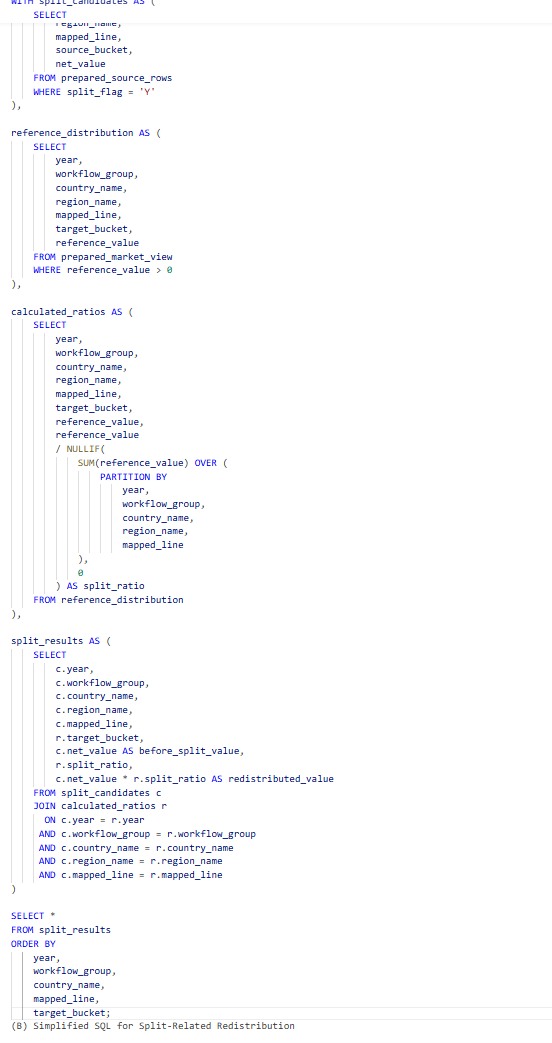
\includegraphics[width=0.85\linewidth]{5.6.4.png}
%     \caption{SQL Fragments for Adjustment- and Split-Related Processing}
%     \label{fig:placeholder}
% \end{figure}




% Frontend development progressed alongside backend reports. Report endpoints return structured JSON data, which is rendered in workflow-specific views. A reusable filterable table component supports column-based filtering and dynamic aggregation, while summary cards, charts, and CSV export provide both detailed and high-level inspection.


% \section{Implementation}

% The prototype was developed incrementally as a full-stack web application. Instead of implementing the final workflow output directly, development first established the technical infrastructure required for authentication, page navigation, CSV upload, structured storage, and staged report generation. This provided the foundation for later workflow-specific logic and frontend inspection.

% The system consists of a React- and TypeScript-based frontend and a Python/FastAPI-based backend. The frontend, built with Vite and React Router, is organized into pages for authentication, matrix submission, upload, workflow navigation, and layer-based inspection. An authentication context manages login state and protected routes, while an API client layer enables consistent communication with backend endpoints.

% \begin{figure}[H]
%     \centering
%     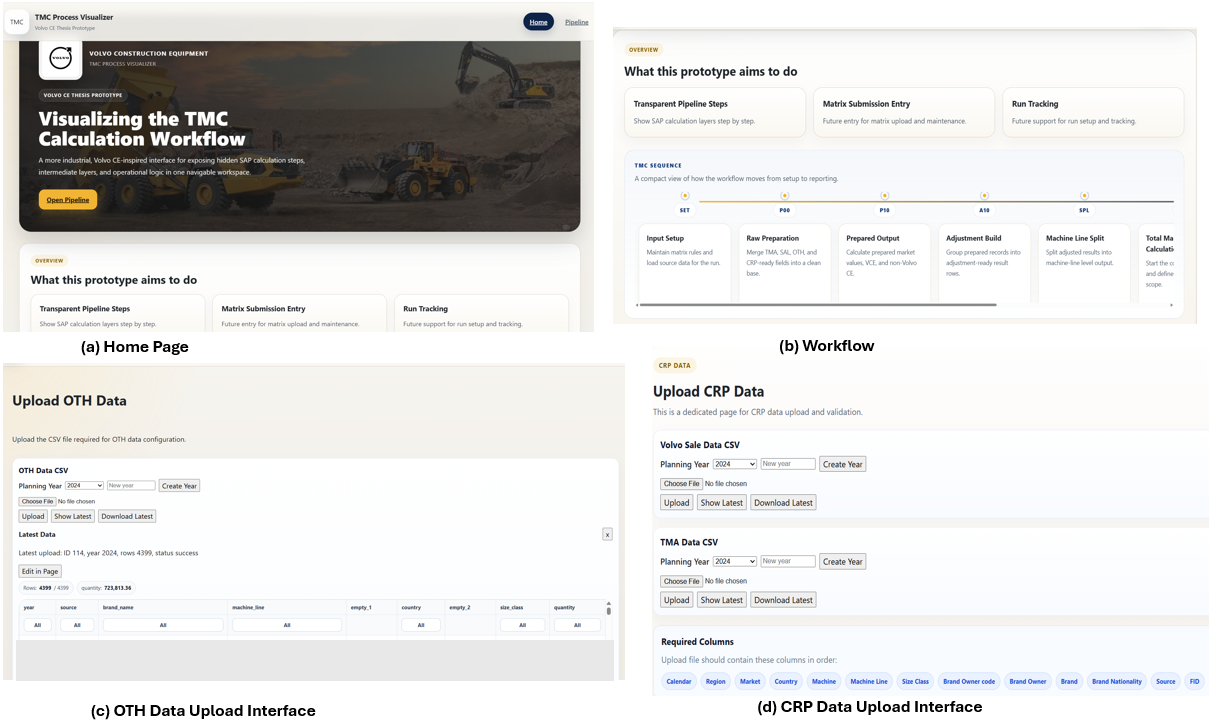
\includegraphics[width=1.1\linewidth]{5.3.1.png}
%     \caption{Selected frontend views developed during the implementation of the prototype}
%     \label{fig:5.3}
% \end{figure}

% On the backend, FastAPI implements the service layer, with a configurable relational data layer that supports SQLite and can be switched to PostgreSQL through environment-based configuration. At startup, the system initializes the workflow and authentication databases and defines separate routers for authentication and workflow-related functionality. These include endpoints for upload, report generation, and result retrieval.

% The next step focused on CSV upload and data storage. Files are submitted from the frontend together with dataset type information and processed by dataset-specific Python handlers. Using \texttt{pandas}, heterogeneous CSV files are parsed, cleaned, and normalized into a consistent structure. The processed rows are stored in the database, while upload metadata is tracked separately so that the latest successful input for each dataset can be reused in later processing steps.

% Once the upload layer was established, development moved to report generation. Initial endpoints produced cleaned source-level outputs for OTH and TMA data, enabling validation of parsing and data alignment.

% \begin{figure}[H]
%     \centering
%     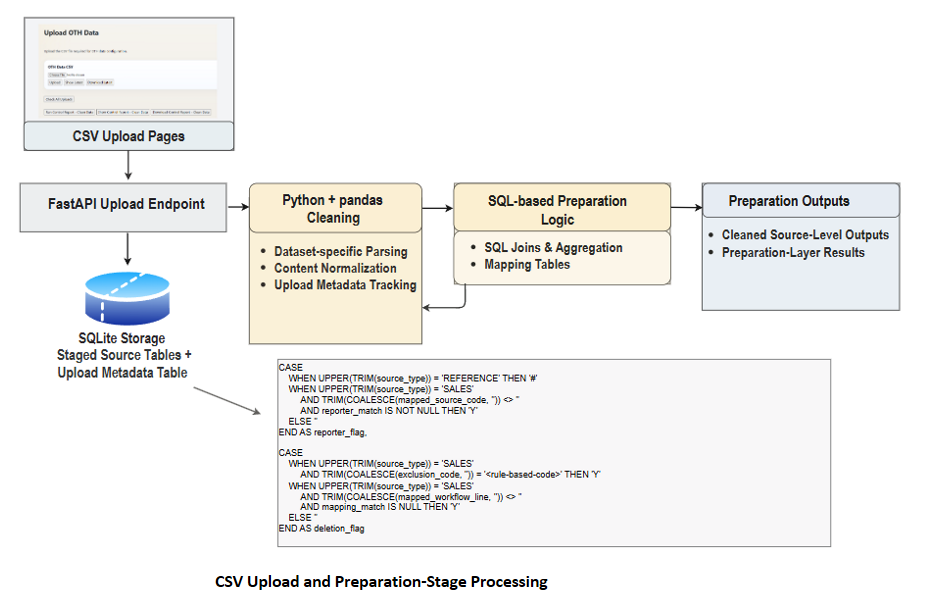
\includegraphics[width=1.1\linewidth]{5.4.png}
%     \caption{Implementation of CSV Upload and Preparation-Stage Processing}
%     \label{fig:5.4}
% \end{figure}

% \begin{figure}[H]
%     \centering
%     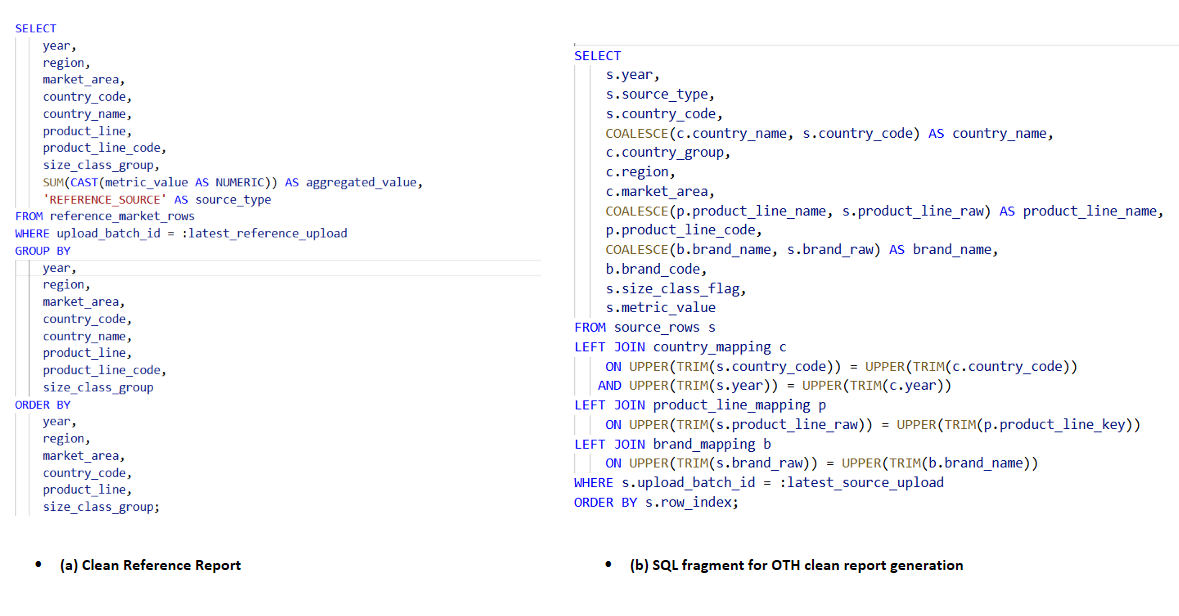
\includegraphics[width=1.1\linewidth]{5.4.1.png}
%     \caption{Simplified SQL Fragments for CRP/TMA and OTH Clean Report Generation}
%     \label{fig:5.4.1}
% \end{figure}

% The preparation stage was then implemented using SQL-based joins, filtering, and aggregation over stored tables. Source records are aligned with mapping data and enriched with workflow control fields such as deletion and reporter flags. The resulting outputs provide a consistent structure for joint inspection of TMA, sales, and OTH data.

% Subsequently, adjustment and prepared result layers were introduced through grouped SQL queries. A key design decision was to return both source-detail rows and derived results within the same output, allowing the frontend to expose how final values are constructed.

% The split stage was implemented by combining prepared OTH data with market-view outputs. Backend logic coordinates the execution, while SQL-derived reference values are used to calculate redistribution ratios. The resulting outputs include summary rows, detailed split results, and supporting reference values, enabling the split logic to be inspected rather than hidden.

% \begin{figure}[H]
%     \centering
%     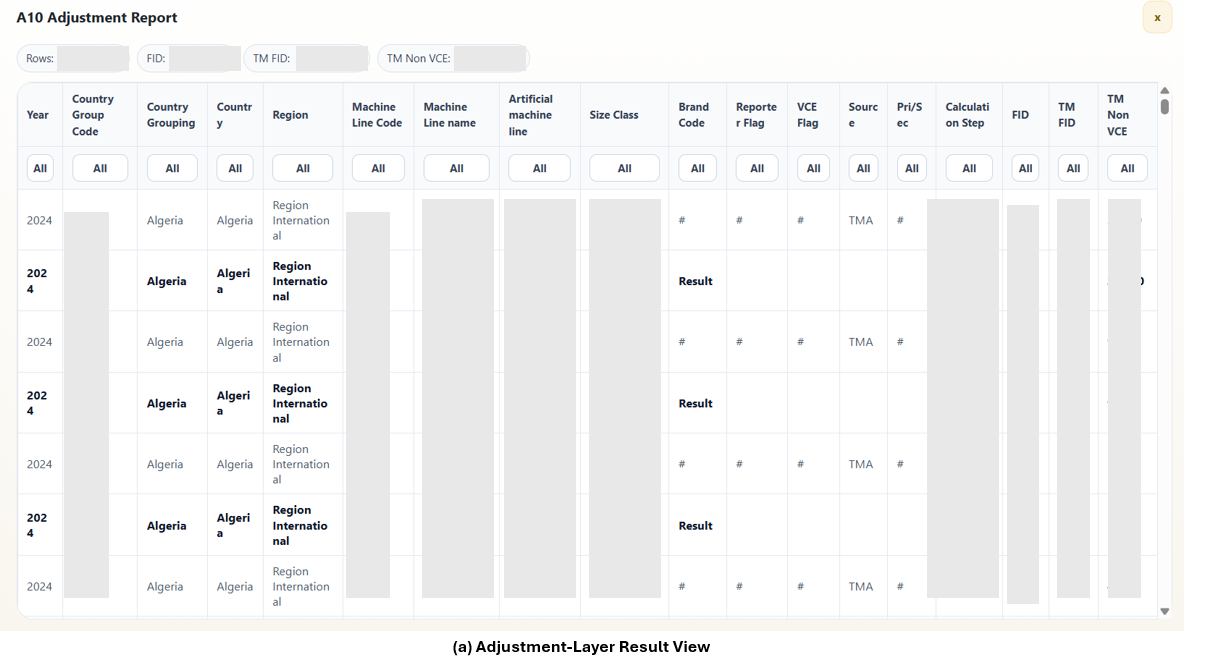
\includegraphics[width=1.1\linewidth]{5.6.1.1.png}
%     \caption{Adjustment-Layer Result View}
%     \label{fig:adjustment-layer-view}
% \end{figure}


% \begin{figure}[H]
%     \centering
%     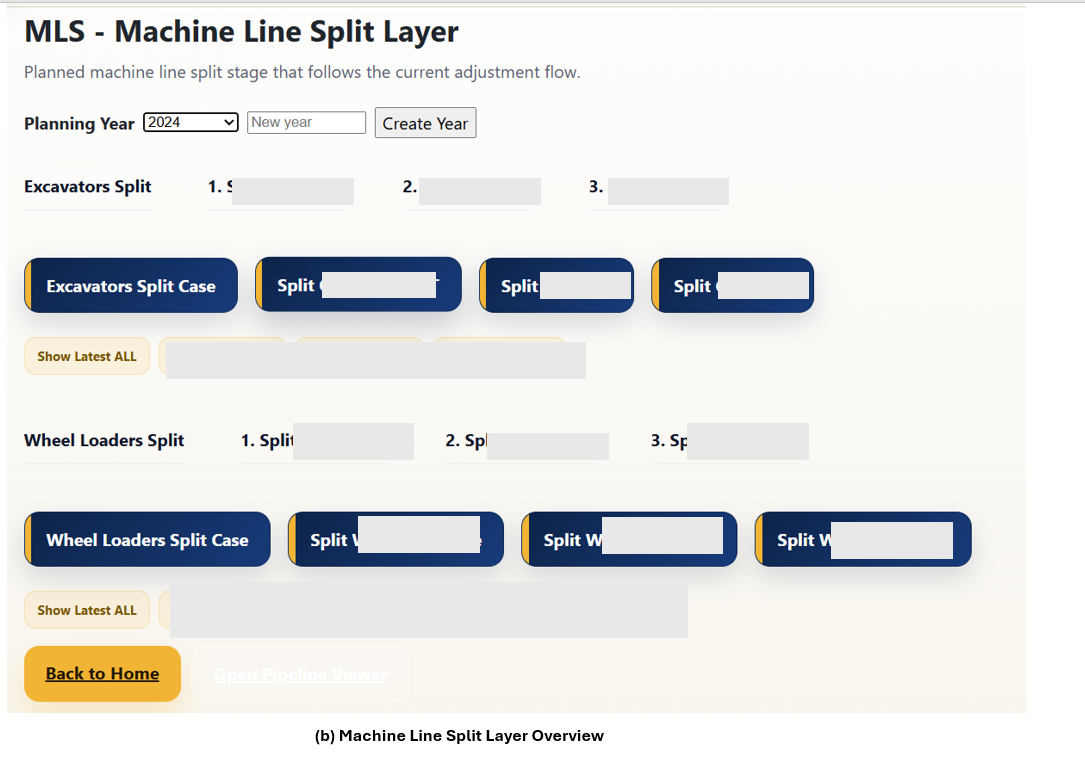
\includegraphics[width=1.1\linewidth]{5.6.1.2.png}
%     \caption{Machine Line Split Layer Overview}
%     \label{fig:split-layer-overview}
% \end{figure}


% \begin{figure}[H]
%     \centering
%     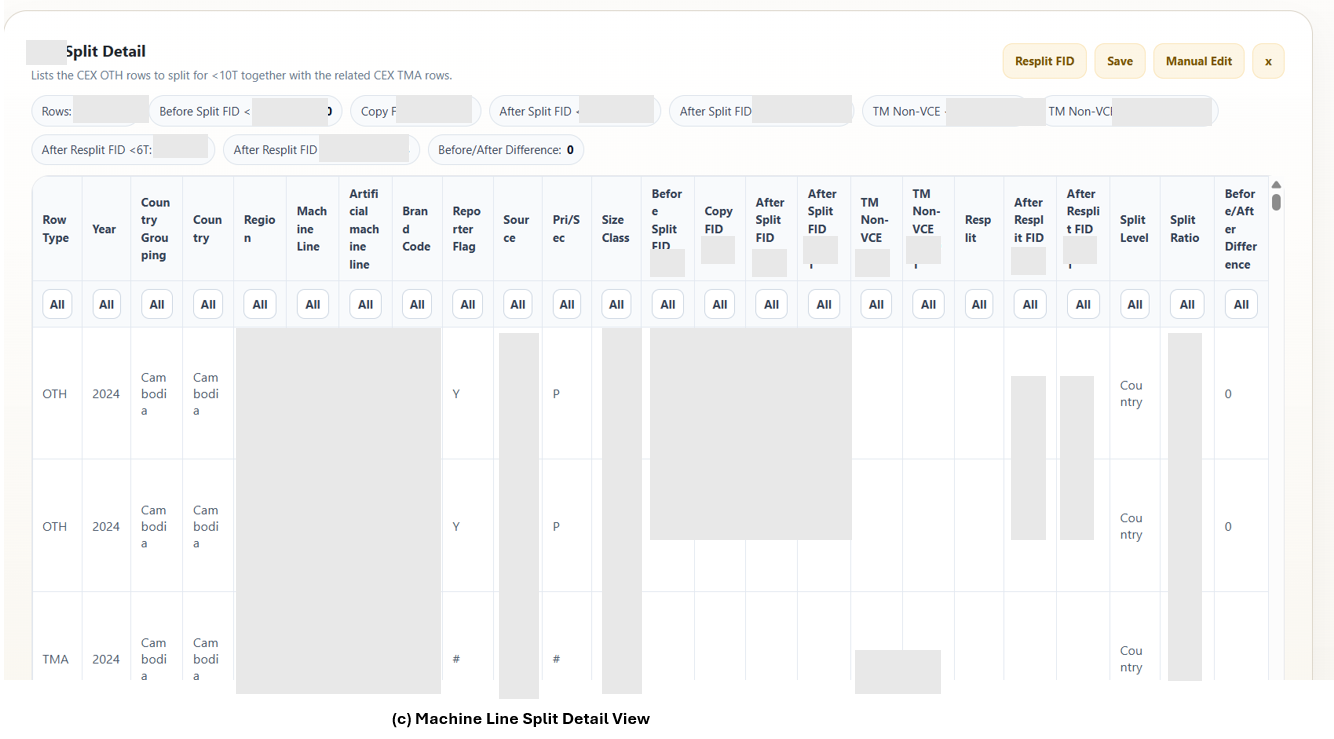
\includegraphics[width=1.1\linewidth]{5.6.1.3.png}
%     \caption{Machine Line Split Detail View}
%     \label{fig:split-detail-view}
% \end{figure}



% \begin{figure}[H]
%     \centering
%     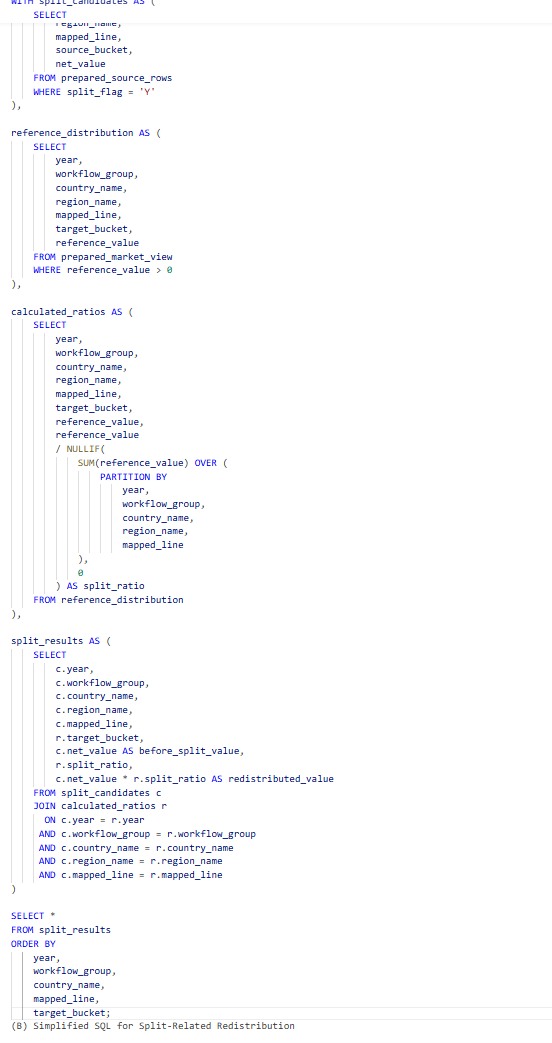
\includegraphics[width=0.85\linewidth]{5.6.4.png}
%     \caption{SQL fragments for adjustment- and split-related processing}
%     \label{fig:sql-fragments-adjustment-split}
% \end{figure}




% Frontend development progressed alongside backend reports. Report endpoints return structured JSON data, which is rendered in workflow-specific views. A reusable filterable table component supports column-based filtering and dynamic aggregation, while summary cards, charts, and CSV export provide both detailed and high-level inspection.


\section{Implementation}

The prototype was implemented as a full-stack web application in which frontend actions trigger backend workflow execution through API-based processing. The implementation followed an incremental structure: authentication, routing, CSV upload, database persistence, and intermediate report generation were established first, after which workflow-specific calculation stages were added. This made it possible to validate each part of the execution chain separately before integrating them into the broader workflow.

At a high level, the frontend acts as the orchestration and inspection layer, while the backend performs data ingestion, workflow processing, and persistence. CSV uploads are normalized into structured relational tables, after which SQL-based transformations and Python-based processing generate preparation, adjustment, and split and resplit outputs. The resulting rows are returned to the frontend as structured JSON and rendered in workflow-specific views for inspection, filtering, aggregation, and export.

\begin{figure}[H]
    \centering
    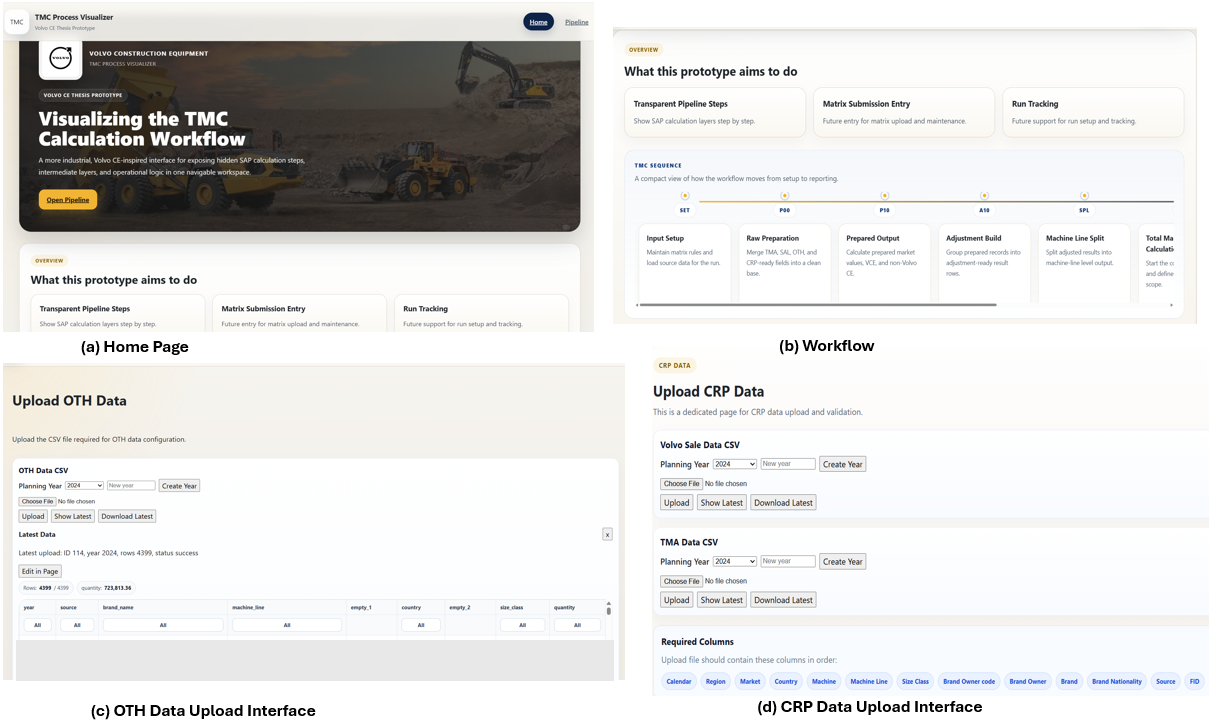
\includegraphics[width=1.05\linewidth]{5.3.1.png}
    \caption{Selected frontend views developed during the implementation of the prototype}
    \label{fig:5.3-main}
\end{figure}

The implementation also established a clear upload-to-processing chain. Files are submitted from the frontend together with dataset type information, processed by dataset-specific handlers, and stored together with upload metadata so that the latest successful input for each dataset can be reused in later workflow steps.

\begin{figure}[H]
    \centering
    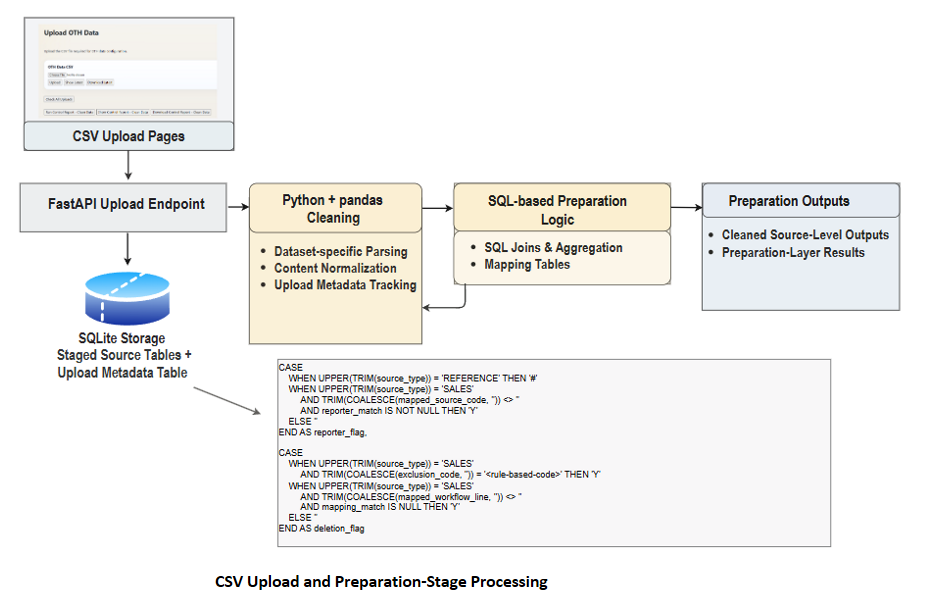
\includegraphics[width=1.05\linewidth]{5.4.png}
    \caption{Implementation of CSV upload and preparation-stage processing}
    \label{fig:5.4-main}
\end{figure}

Once the upload layer was established, the implementation was extended with workflow-specific result layers. In particular, the adjustment and split and resplit views were designed to expose intermediate rows and derived outputs in a form that business users could review directly in the browser.

\begin{figure}[H]
    \centering
    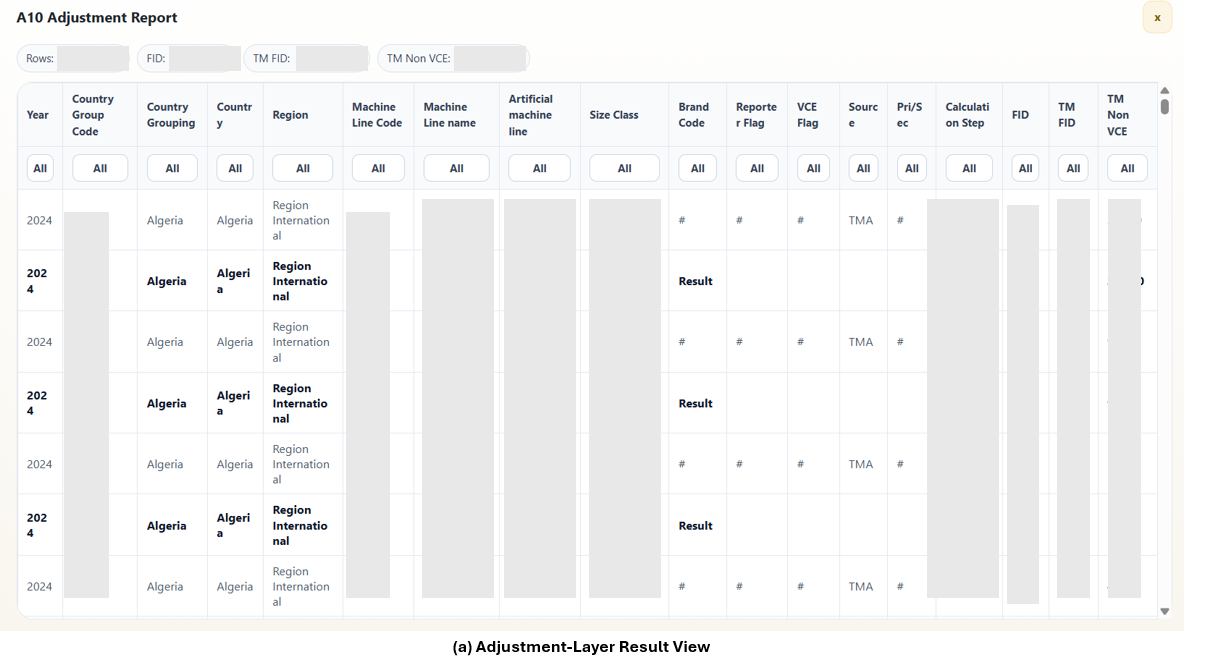
\includegraphics[width=1.05\linewidth]{5.6.1.1.png}
    \caption{Adjustment-layer result view}
    \label{fig:adjustment-layer-main}
\end{figure}

This implementation structure is important because it turns previously embedded workflow logic into explicit and reviewable processing steps. Instead of discussing each technical component in detail in the main body, the thesis focuses here on the design logic and its relation to transparency and inspectability. More detailed implementation notes, example interface views, and supplementary processing fragments are provided in Appendix~\ref{app:supplementary-material}.




